\documentclass[letterpaper,12pt]{article}
\usepackage{array}
\usepackage{threeparttable}
\usepackage{geometry}
\usepackage{mathrsfs}
\geometry{letterpaper,tmargin=1in,bmargin=1in,lmargin=1.25in,rmargin=1.25in}
\usepackage{fancyhdr,lastpage}
\pagestyle{fancy}
\lhead{}
\chead{}
\rhead{}
\lfoot{}
\cfoot{}
\rfoot{\footnotesize\textsl{Page \thepage\ of \pageref{LastPage}}}
\renewcommand\headrulewidth{0pt}
\renewcommand\footrulewidth{0pt}
\usepackage[format=hang,font=normalsize,labelfont=bf]{caption}
\usepackage{listings}
\lstset{frame=single,
  language=Python,
  showstringspaces=false,
  columns=flexible,
  basicstyle={\small\ttfamily},
  numbers=none,
  breaklines=true,
  breakatwhitespace=true
  tabsize=3
}
\usepackage{amsmath}
\usepackage{amssymb}
\usepackage{amsthm}
\usepackage{harvard}
\usepackage{setspace}
\usepackage{float,color}
\usepackage[pdftex]{graphicx}
\usepackage{hyperref}
\hypersetup{colorlinks,linkcolor=red,urlcolor=blue}
\theoremstyle{definition}
\newtheorem{theorem}{Theorem}
\newtheorem{acknowledgement}[theorem]{Acknowledgement}
\newtheorem{algorithm}[theorem]{Algorithm}
\newtheorem{axiom}[theorem]{Axiom}
\newtheorem{case}[theorem]{Case}
\newtheorem{claim}[theorem]{Claim}
\newtheorem{conclusion}[theorem]{Conclusion}
\newtheorem{condition}[theorem]{Condition}
\newtheorem{conjecture}[theorem]{Conjecture}
\newtheorem{corollary}[theorem]{Corollary}
\newtheorem{criterion}[theorem]{Criterion}
\newtheorem{definition}[theorem]{Definition}
\newtheorem{derivation}{Derivation} % Number derivations on their own
\newtheorem{example}[theorem]{Example}
\newtheorem{exercise}[theorem]{Exercise}
\newtheorem{lemma}[theorem]{Lemma}
\newtheorem{notation}[theorem]{Notation}
\newtheorem{problem}[theorem]{Problem}
\newtheorem{proposition}{Proposition} % Number propositions on their own
\newtheorem{remark}[theorem]{Remark}
\newtheorem{solution}[theorem]{Solution}
\newtheorem{summary}[theorem]{Summary}
%\numberwithin{equation}{section}
\bibliographystyle{aer}
\newcommand\ve{\varepsilon}
\newcommand\boldline{\arrayrulewidth{1pt}\hline}


\begin{document}

\begin{flushleft}
  \textbf{\large{Problem Set} 6} \\
  OSM Lab-Math \\
  Sophia Mo
\end{flushleft}

\vspace{5mm}

\noindent\textbf{Problem 1 (8.1)} \\
\begin{center}
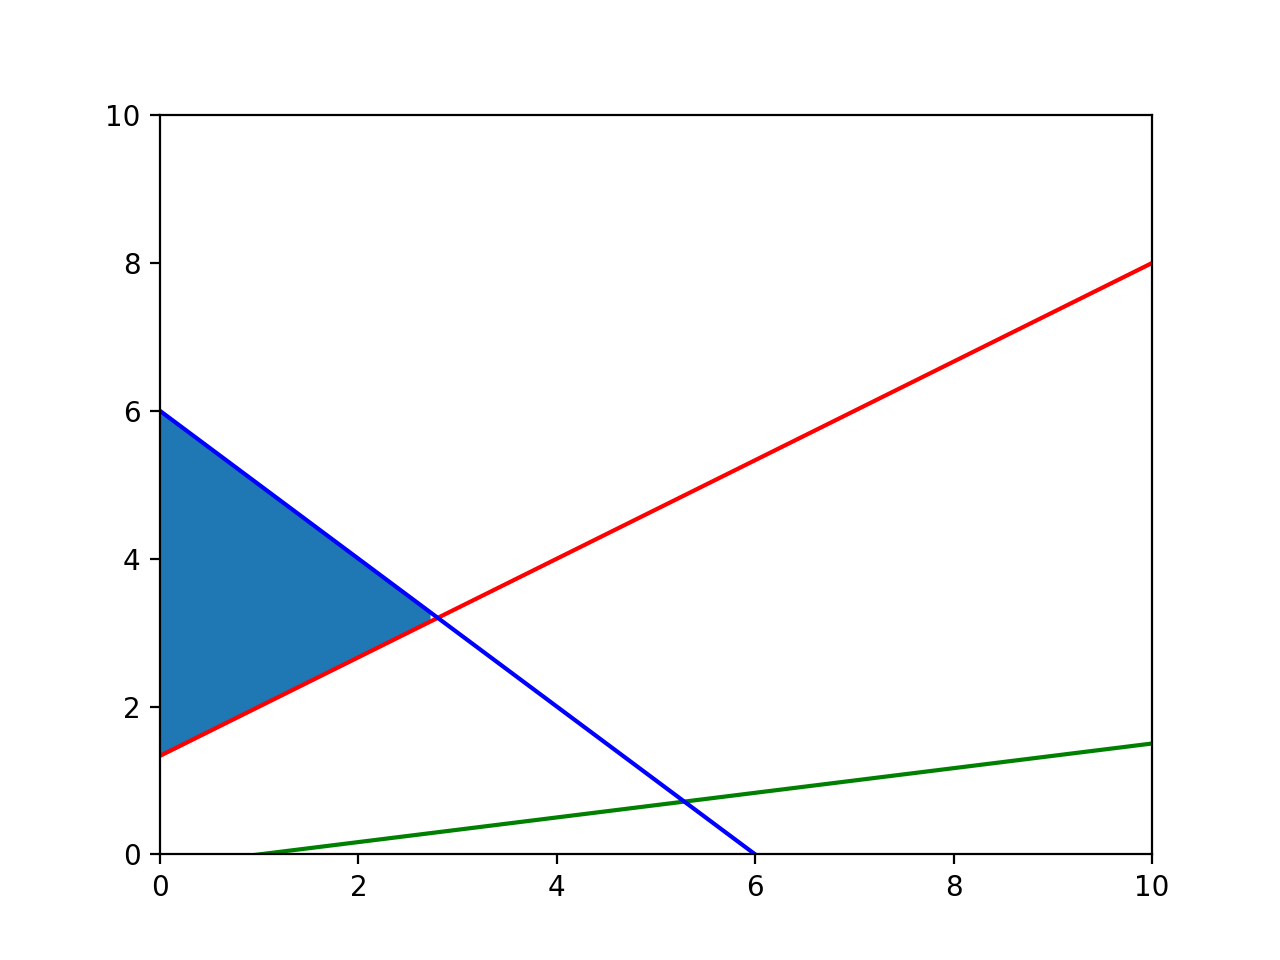
\includegraphics[scale=0.4]{problem_1}
\end{center}
So the optimizer is $ x= \frac{14}{5}, y =\frac{16}{5}$, and the optimal value is $\frac{6}{5}$.\\
\\
\noindent\textbf{Problem 2 (8.2)} \\
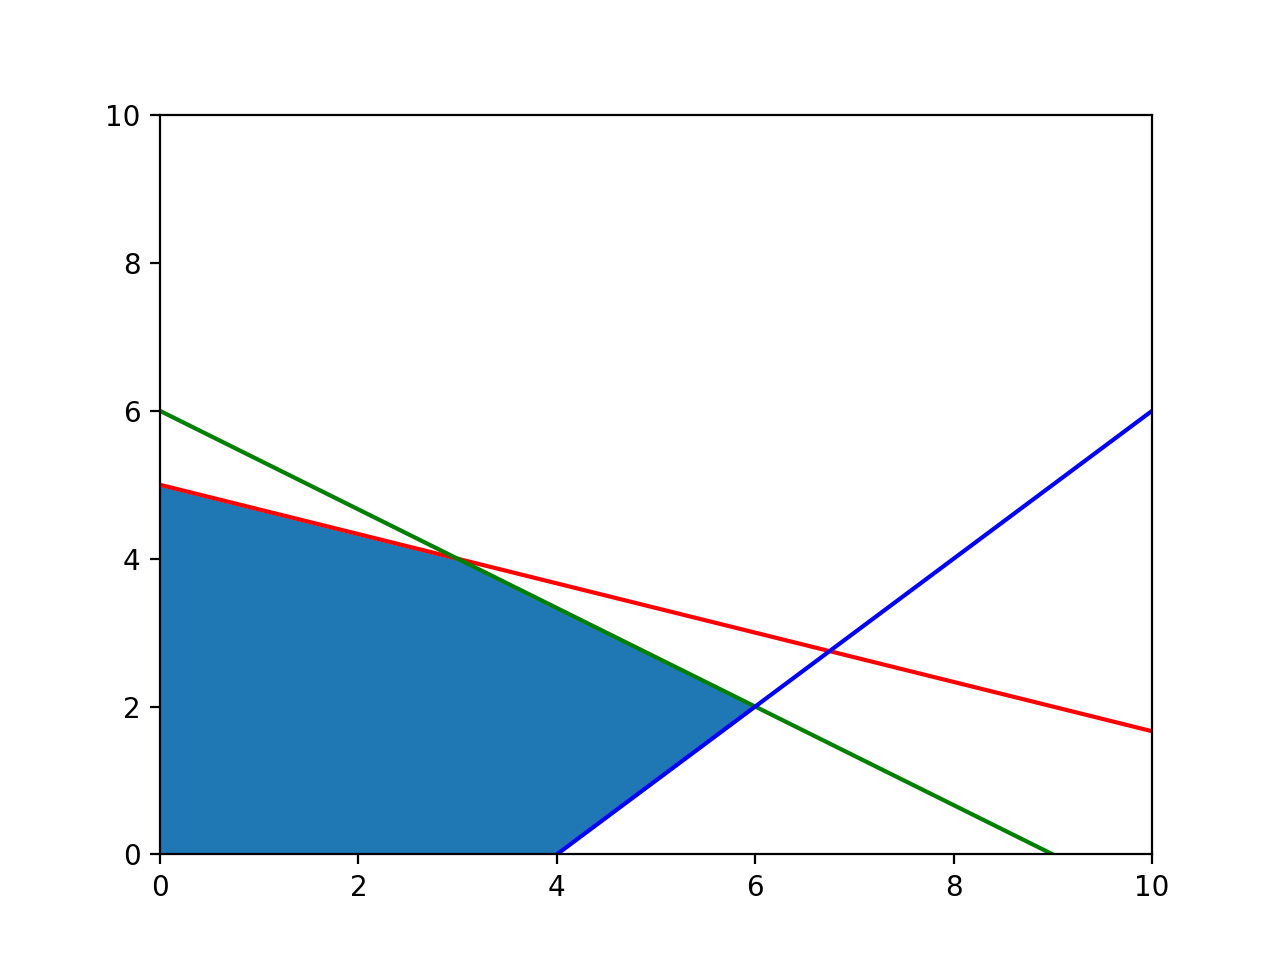
\includegraphics[scale=0.4]{problem_2a}
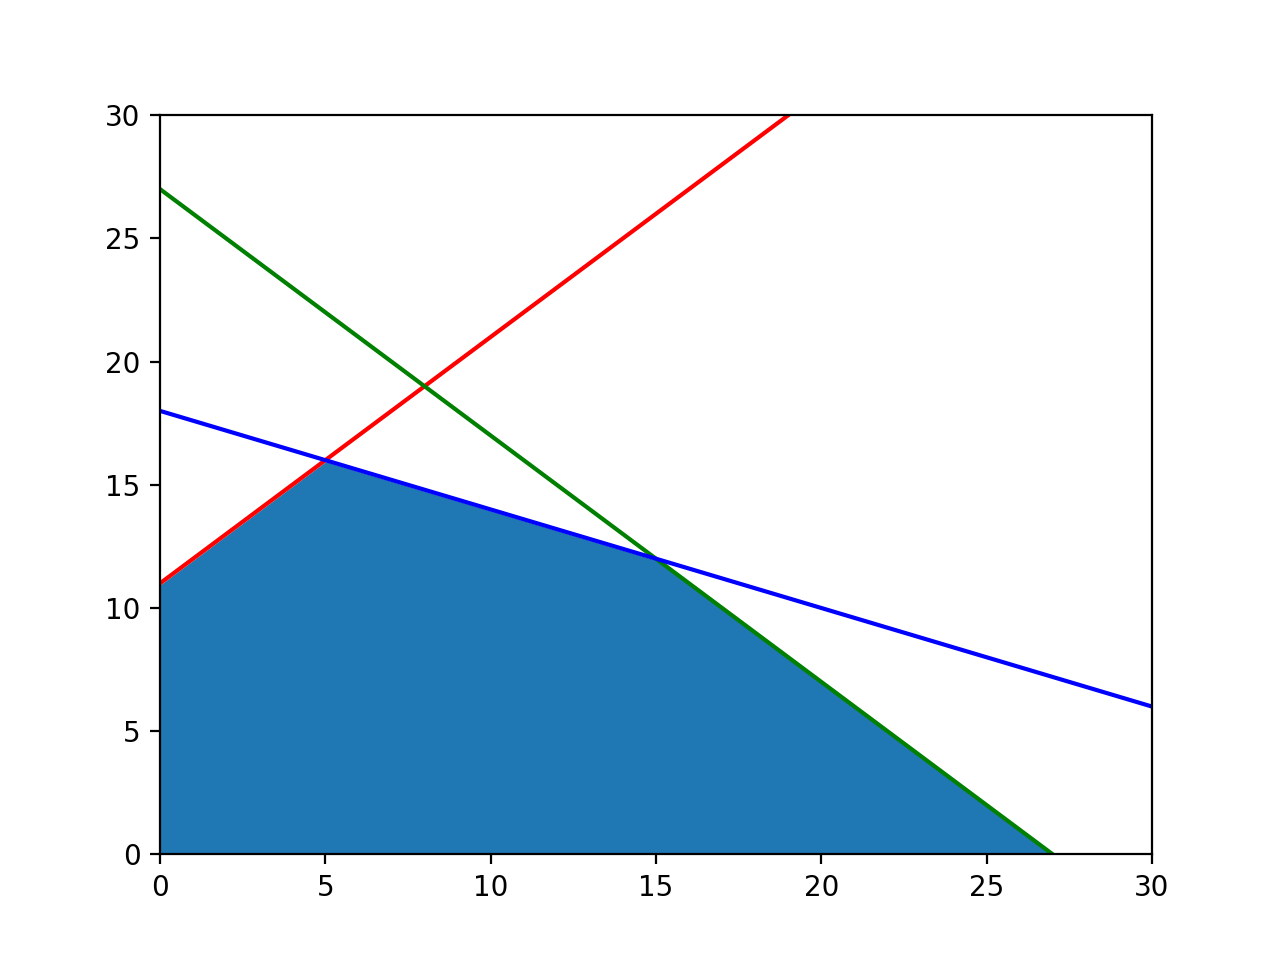
\includegraphics[scale=0.4]{problem_2b}\\
For probelm (i), the optimizer is $ x_1= 6, x_2 =2$, and the optimal value is $20$.\\
For probelm (ii), the optimizer is $ x= 15, y =12$, and the optimal value is $132$.\\
\\
\noindent\textbf{Problem 3 (8.5)} \\
The solutions for the two exercises obtained using the Simplex Algorithm are the same as the one in 8.2.\\
\\
For problem (i), the index after the first pivot is $[2, 3, 0, 4, 1]$, the values are $[11, 10, 4, 0, 0]$.\\
The index after the second pivor is $[2, 1, 0, 3, 4]$, the values are $[3, 2, 6, 0, 0]$.\\
For problem (ii), the index after the first pivot is $[2, 0, 4, 3, 1]$, the values are $[38, 27, 36, 0, 0]$.\\
The index after the second pivor is $[2, 0, 1, 3, 4]$, the values are $[14, 15, 12, 0, 0]$.\\
\\
\noindent\textbf{Problem 1 (8.7)} \\
(i)\\
The optimizer is $x_1 = 3$, $x_2=4$, and the optimal value is $11$.\\
\\
(ii)\\
The problem is infeasible because by combining the second and third constraints, we get $x_1<0$, which contradicts the constraint that $x_1\geq 0$.\\
\\
(iii)\\
The optimizer is $x_1 = 0$, $x_2=2$, and the optimal value is $2$. \\
\\
\noindent\textbf{Problem 1 (8.13)} \\
Suppose that $x=0$ is not an optimal point, then the optimal value of both the primal and the dual problems should be positive. Since the dual problem takes the form:\\
min $0$\\
s.t. $A^Ty \geq c, y\geq0$, we know the dual problem is infeasible. So the primal is unbounded.\\
Suppose that the linear problem is bounded, then the dual problem should be feasible. It follows that the primal problem has an optimal value of 0. For this to hold, $x=0$ must be an optimal point.\\
\\
\noindent\textbf{Problem 1 (8.17)} \\
Suppose the primal problem is:\\
max $c^Tx$\\
s.t. $Ax\leq b, x\geq 0$.\\
Then the dual problem is :\\
min $b^Ty$\\
s.t. $A^Ty\geq c, y\geq 0$, which is equivalent to :\\
max $(-b^T)y$\\
s.t. $(-A^T)y\leq -c, y\geq 0$\\
The dual of the dual problem is then:\\
min $(-c^T)x$\\
s.t. $(-A)x\geq -b, x\geq 0$, which is equivalent to the primal problem.\\
\\
\noindent\textbf{Problem 1 (8.18)} \\
Solve by the Simplex Algorithm, we know the optimizer for the primal problem is $x_1 = 1.25, x_2 = 0.5$, and the optimal value is $1.75$. The dual problem is: \\
\\
min\begin{center}
$3y_1+5y_2+4y_3$
\end{center}
s.t.
\begin{align*}
2y_1+y_2+2y_3\geq 1\\
y_1+3y_2+3y_3\geq 1\\
y_1, y_2, y_3 \geq 0
\end{align*}
The optimizer for the dual problem is $y_1=\frac{1}{4}, y_2=0, y_3 = \frac{1}{4}$, and the two problems have the same optimal value.

\end{document}
